\documentclass[tikz]{standalone}
\usetikzlibrary{arrows.meta}
\usepackage{mathtools}
\usepackage{amssymb}
\begin{document}
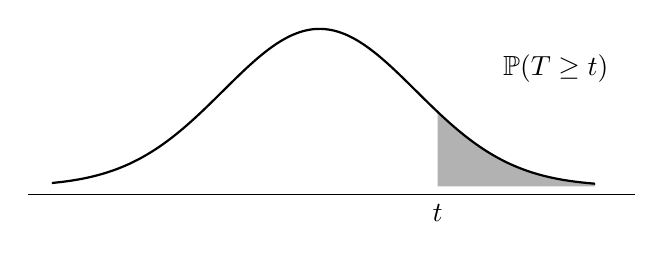
\begin{tikzpicture}[>={Stealth[length=6pt]},
  declare function={g(\x)=2*exp(-\x*\x/3);
    xmax=3.5;xmin=-3.4;x0=1.5;ymax=2.75;}]
 \draw[black] (-3.7,-0.1) edge[-] (4,-0.1);
 \fill[gray!60] plot[domain=x0:xmax,samples=15,smooth] (\x,{g(\x)}) -- (xmax,0) -| cycle;    
 \draw[thick] plot[domain=xmin:xmax,samples=51,smooth] (\x,{g(\x)}); 
 \path (x0,-0.1) node[below]{\(t\)} (3, 1.2) node[above]{\(\mathbb{P}(T \geq t)\)};
\end{tikzpicture}
\end{document}